% This document is part of the FlatLikelihoodFlatPrior project.
% Copyright 2024 the author. All rights reserved (for now).

% to-dos and questions
% --------------------
% - should I generalize to more than one important parameter? Or just discuss it at the end?
% - I am using first-person singular everywhere. Okay?
% - Should I be more careful about using LF and Likelihood consistently? Audit.

\documentclass[10pt]{article}
\usepackage[letterpaper]{geometry}
\usepackage{graphicx} % Required for inserting images

% hogg typesetting issues
\usepackage{setspace}
\setstretch{1.08}
\setlength{\textwidth}{5.00in}
\setlength{\oddsidemargin}{3.25in}
\addtolength{\oddsidemargin}{-0.50\textwidth}
\setlength{\textheight}{8.70in}
\setlength{\topmargin}{-0.20in}
\pagestyle{myheadings}
\markboth{foo}{Hogg / Flat likelihood, flat prior, peaked posterior}
\frenchspacing

% text macros
\newcommand{\foreign}[1]{\textsl{#1}}
\newcommand{\figref}[1]{\figurename~\ref{#1}}

% hogg math issues
\usepackage{amsmath, mathrsfs}
\newcommand{\given}{\,|\,}
\newcommand{\norm}[1]{\left\lVert{#1}\right\rVert}
\newcommand{\dd}{\mathrm{d}}

\title{\bfseries Flat likelihood, flat prior, peaked posterior}
\author{Hogg}
\date{September 2024}

\begin{document}

\maketitle

\paragraph{Abstract:}
I present an example likelihood function that is flat:
It has no peak in any of the $p$ parameters on which it depends, although it is peaked in certain linear combinations of the $p$ parameters.
The data are compatible with any value of any individual parameter; the profile likelihood is flat for every one of the $p$ parameters.
I present a prior that is also flat:
It is the outer product of $p$ uniform distributions.
When this likelihood function is multiplied by this prior, every marginal posterior and every marginal likelihood, for every one of the $p$ parameters (and indeed almost all linear combinations of the $p$ parameters), is peaked, and usually not at or near an edge of the prior range.
Fundamentally the problem is that the shape of the uniform prior isn't aligned with the degeneracy surface in the likelihood, so the effective volume of the prior is very different in regions of identical likelihood value.
This example shows that a posterior peak doesn't indicate a successful measurement, and that flat priors are in fact informative, especially under marginalization and especially when the number of parameters is large (like $>3$).
Simple prior-dependence tests can diagnose these issues.

\section{Introduction}
Even if the goal of \emph{the scientific enterprise} is to update a continuously evolving, community-level, posterior pdf over every theory in play and over every parameter of every theory in play, the goal of \emph{an individual scientific paper} might not be to produce a posterior.
If your personal goal is to update your own posterior pdf on some parameters, you can take data, make a likelihood function, and multiply it by your prior pdf (your posterior pdf from before you took these data, maybe).
That's a bad goal, however, if you are a scientist.
Scientists are expected to update \emph{everyone's} posterior pdfs, not just their own.
You can only update someone else's posterior pdf by providing that person with a likelihood function.
The key idea of Bayesian reasoning is that posterior pdfs are only updated by data through multiplication by a likelihood function (and renormalization).

Indeed, frequentists and Bayesians agree on something very important,
which is the \emph{likelihood principle}:
The likelihood function contains all the information in the data about the parameters.
The likelihood function is a probability density function (pdf) for the data, given parameters.
Once data are taken, the data are fixed and this function can be seen as a function of the parameters.
This function is sufficient:
Everything that the data can tell you about the parameters is contained in the likelihood function.
That's why, for Bayesians, the likelihood function is what's used to update your beliefs, given new data.
It's also why the likelihood function appears in frequentist theorems about optimal estimators and optimal decision criteria.

Sometimes frequentists and Bayesians like to disagree.
One point on which they sometimes disagree, but on which they should not, is \emph{subjectivity}.
Both frequentist and Bayesian data analyses are always, technically, subjective.
The reason is: The construction of a likelihood function involves making choices, and those choices are made by the investigators who make them.
So please don't see what comes below as a battle between subjectivity and objectivity; we are all doing our subjective science here.
The sense in which the scientific enterprise is objective is that scientists can agree that if they make the same choices, then they will get the same answers.
That's the only sense of objectivity to which we can aspire, here or anywhere.

\paragraph{My contributions:}
I show that even when the likelihood is flat (in the relevant sense), and even when the prior is flat (in every sense), the marginalized posterior pdf can nonetheless show a peak.
I show that this situation is generic when the number of nuisance parameters is more than a few.
I show that this situation is easily diagnosed either by computing profile likelihoods (when the number of nuisance parameters is small) or by testing the prior dependence of the posterior (when the number of nuisance parameters is large).

\paragraph{Prior work:}
There is nothing really new about these results.
They are all simple consequences of prior-volume effects or prior-edge effects discussed in many places (CITE THINGS).
This demonstration also links to the idea that flat priors aren't in fact uninformative, as has been argued elsewhere in many places (CITE THINGS).

\section{Problem setup}
The idea is that we have data $Y$ of some shape and size that we don't need to precisely specify.
We have parameters $\theta$, which make up a $p$-vector, or an ordered list of $p$ elements.
If we use the symbol $\theta_i$ to denote the $i$th element ($1\leq i\leq p$) of this vector, we could say that $\theta_1$ is the ``important parameter'' that we care about and the other $\theta_i$ (for $i>1$) are ``nuisance parameters'' that we don't care about.
This split of parameters into important and nuisances won't be essential to the argument.

It turns out that the physics of the problem---the way that the world generates data $Y$ in our model---is quite complicated, but we are able nonetheless to write a computer program that can compute values of the likelihood function $p(Y\given \theta,\mathscr{I})$.
The likelihood function (LF) is the pdf for the data $Y$ given parameters $\theta$, with the symbol $\mathscr{I}$ standing in for all of the assumptions going in to the model.
Technically the LF is the pdf for the data given the parameters \emph{evaluated at the value of the observed data}.
This is what our computer program computes for us.

It turns out (but this is not transparent to us) that, when evaluated at the observed data $Y$, the LF depends only on certain linear combinations of the parameters $\theta$.
That is, there is a rectangular $q\times p$ matrix $A$, with $q<p$, such that, to some very good approximation,
\begin{align}
    \ln p(Y\given\theta,\mathscr{I}) &= K - \frac{1}{2}\,\norm{A\cdot\theta - a}^2 ~,\label{eq:LF}
\end{align}
where $K$ is a scalar constant, $a$ is a $q$-vector constant, and the norm is the standard euclidean norm (square root of sum of squares).
Presumably the story would be different for different data, because $K, A, a, q$, and even the linearity might all depend strongly on $Y$.
But $Y$ is the data we have.
Note that here and everywhere, vectors like $\theta$ and $a$ are column vectors.

Just to be clear, the LF \eqref{eq:LF} is Gaussian-shaped in $q$ directions in the parameter space, and completely degenerate or uniform in all orthogonal directions.
It can be seen as being a finite-width hypersurface that is $p-q$ dimensional in its large (infinite) dimensions, and has a finite Gaussian thickness in the remaining $q$ dimensions.

Now the question is, given this LF: \emph{Is the parameter of importance constrained by these data?}
Since we all agree on the likelihood principle, that is, that the likelihood function is sufficient with respect to the data,
the answer to this question is somehow tied up with the properties of the $A$ matrix.
The $A$ matrix can be thought of as projecting the parameter space into a $q$-dimensional linear subspace of the full $p$-dimensional parameter space (and then applying some affine transformation)
Therefore, the data constrain parameter $\theta_1$ if and only if any vector in the parameter space pointing purely in the $\theta_1$ direction lies precisely in the $q$-dimensional subspace spanned by the $A$ matrix.
If we think of the rectangular matrix $A$ as being generated by some kind of arbitrary process, this is very unlikely \foreign{a priori}.
So in general the answer to this question will be ``no.''
The data do not constrain the parameter of importance.

When we do Bayesian inference, we will want a prior, and, because we want to be maximally uninformative, we will choose a prior that is precisely flat in all parameters $\theta_i$.
That is
\begin{align}
    p(\theta\given\mathscr{I}) &= \prod_{i=1}^p U(\theta_i\given a_i, b_i) \\
    U(x\given a, b) & = \left\{\begin{array}{cl}
    0 & \mbox{for $x<a$,} \\
    (b-a)^{-1} & \mbox{for $a<x<b$,} \\
    0 & \mbox{for $b<x$,}\end{array}\right.
\end{align}
where the $a_i, b_i$ ($1\leq i\leq p$) are prior limit parameters with $a_i<b_i$ for all $i$.
In fact, these flat priors \emph{aren't} uninformative (CITE THINGS), but perhaps, in some circumstances, they are least informative?
It turns out that they will be quite informative in what follows.
This prior requires us to make $2\,p$ choices, to wit, the upper and lower limits $a_i, b_i$ for each parameter $\theta_i$.

Now we define the basic tools of frequentist and Bayesian inference:
\begin{itemize}
\item
The \emph{maximum likelihood estimator} is the location in parameter space that optimizes the LF.
In this case, when $q<p$, there is no such point.
Instead there is a $(p-q)$-dimensional parameter subspace that is all tied for maximum likelihood.
Thus there is no maximum-likelihood estimator for this problem.
\item
The \emph{profile likelihood} for the important parameter $\theta_1$ is the maximum possible likelihood value for each setting of parameter $\theta_1$, optimizing over all the nuisance parameters $\theta_i$ ($i>1$).
In our simple setup, when $q<p$ and $A$ is generic, this will be exactly $K$ for any value of $\theta_i$.
That is, in this problem, the profile likelihood is flat with respect to $\theta_1$ (or indeed any parameter $\theta_i$).
The profile likelihood is a prior-free (and hence frequentist-safe) way of eliminating nuisance parameters.
\item
The \emph{posterior pdf} $p(\theta\given Y,\mathscr{I})$ is the product of the prior pdf and the likelihood, renormalized
\begin{align}
    p(\theta\given Y,\mathscr{I}) &= \frac{1}{Z}\,p(Y\given\theta,\mathscr{I})\,p(\theta\given\mathscr{I}) ~,
\end{align}
where $Z$ is a normalization constant (sometimes called ``the evidence'').
Because, in this problem, the likelihood is flat (in some $q$-dimensional linear subspace) and the prior is flat, the posterior will also be flat (in that same $q$-dimensional linear subspace).
\item
The \emph{marginal posterior pdf} is the posterior pdf for the important parameter $\theta_1$, found by integrating the full posterior pdf over all the the nuisance parameters $\theta_i$ ($i>1$).
\begin{align}
    p(\theta_1\given Y,\mathscr{I}) &= \int_{a_2}^{b_2}\int_{a_3}^{b_3}\cdots\int_{a_p}^{b_p} p(\theta\given Y,\mathscr{I})\,\dd\theta_2\,\dd\theta_3\cdots\dd\theta_p ~.
\end{align}
In my world, this integration is usually done by Monte Carlo, or even Markov chain Monte Carlo (CITE THINGS), so it is done approximately.
That is how we will proceed below (even though in this simple setup, the integrals can probably be written explicitly in terms of erfs).
\item
The \emph{marginal likelihood} is very similar to the marginal posterior pdf, but we don't put any prior on the important parameter; we only put the priors on the nuisance parameters.
Since, in the problem considered here, the prior on $\theta_1$ is both flat and separable from the priors on the nuisance parameters, the marginal likelihood is identical in shape to the marginal posterior pdf, so we will only consider the marginal posterior pdf in what follows.
\end{itemize}

In the experiments that follow, we will choose the integers $p, q$ and generate the matrix $A$ and the vector $a$ randomly.
We will then set prior bounds for each of the parameters $\theta_i$ and compute marginal posteriors for $\theta_1$.
Without loss of generality, we can set the scalar constant $K=0$ always, because only likelihood ratios---only differences in log likelihood---matter to the inferences.

\section{Experiments and results}
\paragraph{Experiment 1:}
In Experiment~1, I choose $p=6$ and $q=2$ to demonstrate the basic properties of the problem.
I set the $q\times p$ matrix $A$ to be a pair of randomly generated orthogonal unit $p$-vectors.
These are made by generating $q$ vectors randomly from an isotropic multivariate normal, and then running Gram--Schmidt orthonormalization.
The vector $a$ is chosen randomly (and is truly arbitrary).
Because the vectors in $A$ are normalized, the width of the degenerate likelihood surface is unity in the sense of a Gaussian standard deviation.

Importantly, in this Experiment, I choose the prior limits $a_i, b_i$ (for all $1\leq i\leq p$) such that some region of high likelihood passes near (but not exactly at) the center of the prior hyper-box.
For each of $M=12$ trials, I draw $N=2^15$ samples iid from the prior, and use them to compute an estimate of the marginal posterior pdf for each of the parameters $\theta_i$ ($1\leq i\leq p$).
That provides $M=12$ (noisy) estimates of the marginal posterior pdf for each of the $p=6$ parameters.

These estimates of the marginal posterior pdfs are shown in \figref{fig:Experiment1}.
Several of the panels of this \figurename{} show clear peaks in the posterior pdf, even though \emph{neither the LF nor the prior pdf are peaked in any parameter}.
\figref{fig:Experiment1} is the key plot; it delivers the fundamental punchline of this investigation.
\begin{figure}[t!]
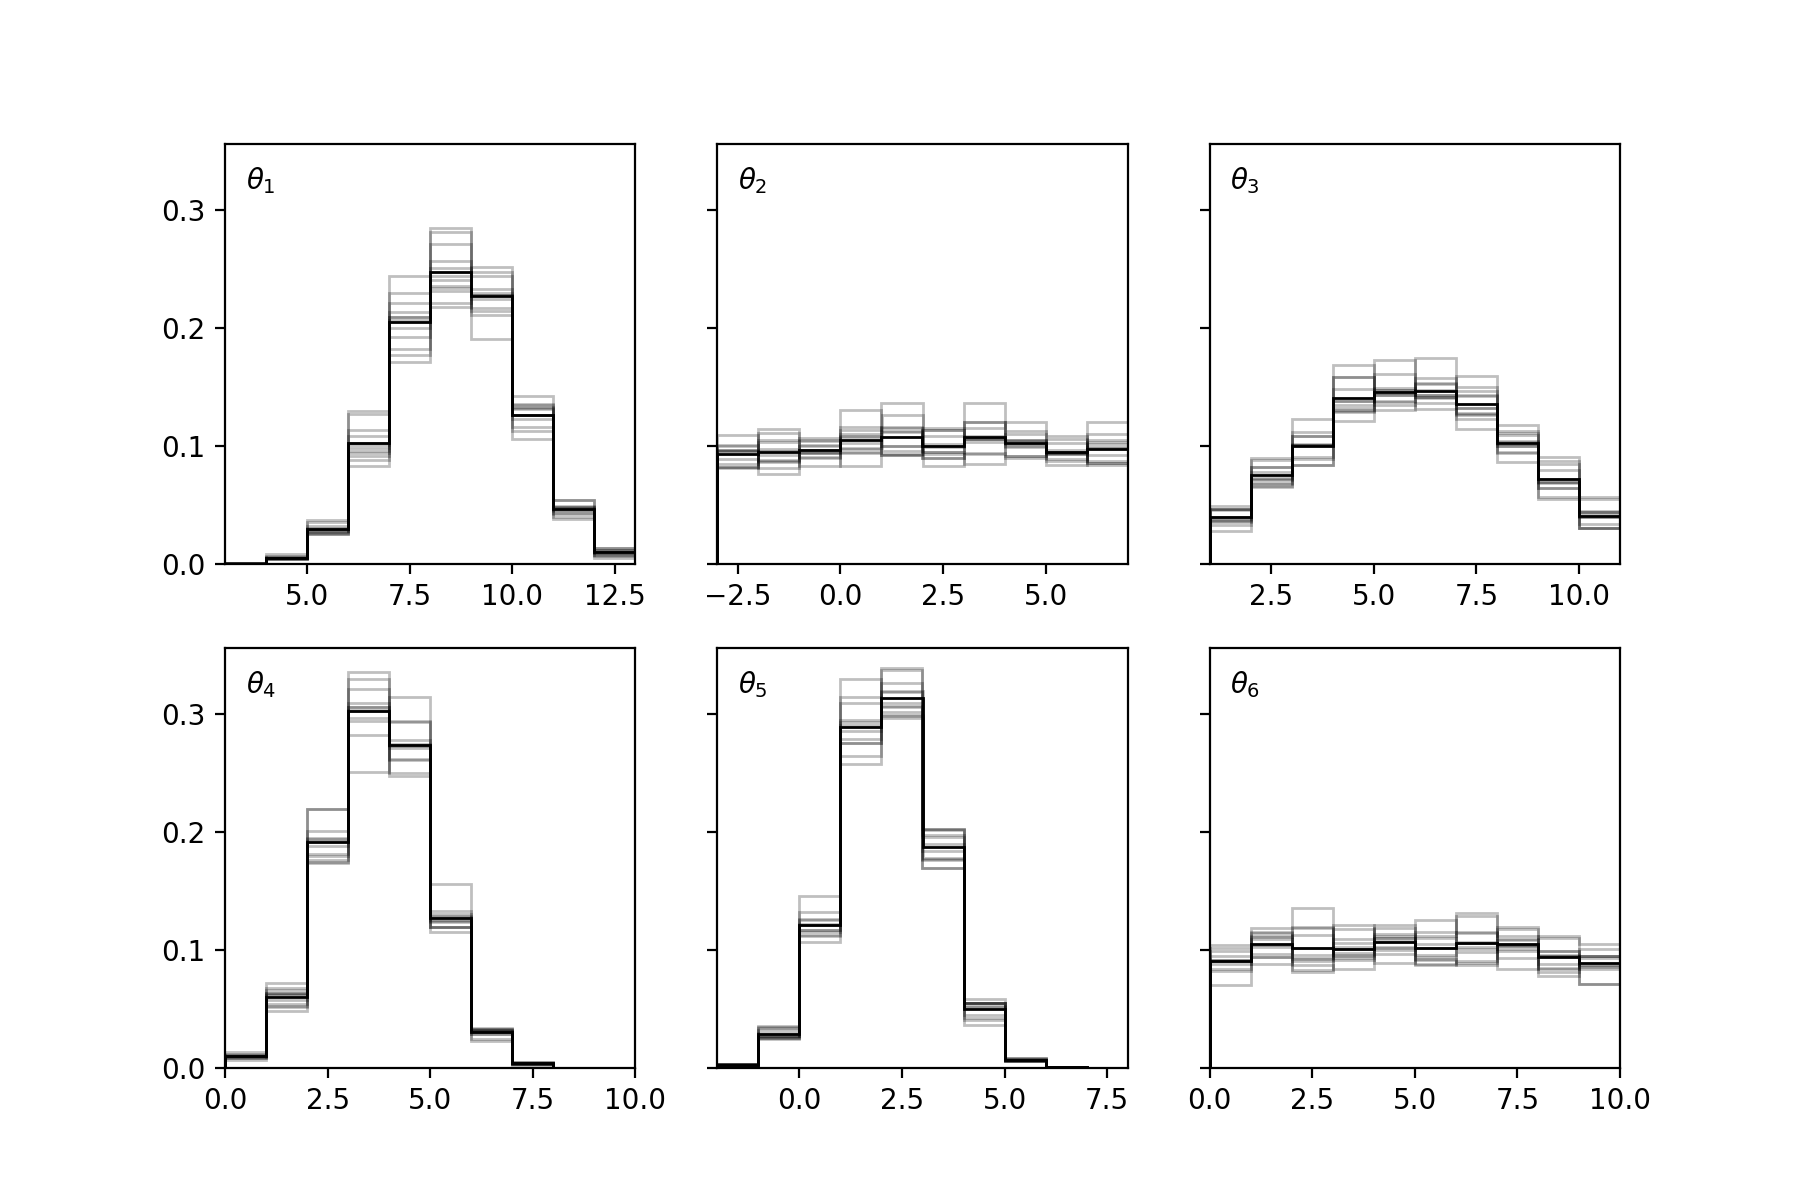
\includegraphics[width=\textwidth]{./notebooks/Experiment1.png}
\caption{Estimates of the marginal posterior pdfs for all parameters $\theta_i$ ($1\leq i\leq 6$). Each panel shows 12 estimates (grey lines) of the marginalized posterior pdf for one of the parameters, and the average of the 12 estimates (black line). Each of the 12 estimates was obtained my a Monte Carlo sampling with $N=2^15$ samples drawn iid from the prior pdf. Each panel $i$ has limits $a_i, b_i$ corresponding to the limits on the prior for parameter $\theta_i$.\label{fig:Experiment1}}
\end{figure}

\section{Discussion}

HOGG: Summarize results

HOGG: Explain \emph{why} this is happening. It's all about volume!

HOGG: Explain why you want to do profile likelihood, in general.

HOGG: Explain why you can't do profile likelihood, in general.

HOGG: Say that this project may seem artificial, but it looks a lot like Villaescusa et al.

HOGG: Did anything depend on there being only one important parameter? No! Demonstrate.

HOGG: It is important to show that claims about the data can be justified in terms of the likelihood.

\paragraph{Acknowlegements:}
It is a pleasure to thank
  Gaby Contardo ()
for valuable discussions.
The Flatiron Institute is a division of the Simons Foundation.

% HOGG: Bibliography

\end{document}
